\documentclass[a1paper, portrait]{baposter}

\definecolor{base00}{RGB}{101,123,131}
\definecolor{base2}{RGB}{238,232,213}
\definecolor{base3}{RGB}{253,246,227}

\definecolor{yellow}{RGB}{181,137,0}
\definecolor{red}{RGB}{220,50,47}
\definecolor{magenta}{RGB}{211,54,130}

\usepackage[utf8]{inputenc}
\usepackage{tikz}
\usepackage{url}
\usepackage{titling}
\usepackage{epstopdf}

\usepackage{xspace}
\newcommand{\SPRAY}[0]{\textsc{Spray}\xspace}
\newcommand{\LSEQ}[0]{\textsc{LSeq}\xspace}
\newcommand{\CRATE}[0]{\textsc{Crate}\xspace}

\newcommand{\BOLD}[1]{\textcolor{red}{\textbf{#1}}}

\title{\CRATE: Writing Stories Together with our Browsers}
\author{Brice Nédelec, Pascal Molli, Achour Mostefaoui}

\begin{document}
\begin{poster}{
    grid=false,
    bgColorOne=white,
    bgColorTwo=white,
    linewidth=1pt,
    columns=3,
    %%
    headershape=roundedright, 
    headerheight=0.18\textheight,
    headerborder=open,
    headerColorOne=base3,
    headerColorTwo=base2,
    borderColor=yellow,
    eyecatcher=false,
    %%    
    textborder=rectangle,
    boxColorOne=base2,
    boxColorTwo=base2,
    textfont=\sffamily
  }
  {}
  {\huge\textsc{\thetitle}\vspace{0.4em}}
  {\theauthor \\ \url{first.last@univ-nantes.fr}}
  {
\includegraphics[height=0.16\textheight, interpolate=false]{logos/crateicon.png}}

  \headerbox{\textsc{Distributed Collaborative Editors}}
  {name=context, column=0, span=3, row=0} {
    Distribute the work across space, time, organization.\\
    Improve the commitment of users, and the quality of documents.\\
    \\
    Centralized solutions: \\
    - Raise privacy issues, for the mediator of the editing session can
      observe all users and documents; \\
    - Scalability issues, for one server must handle the load of all users. \\
    \\
    Decentralized solutions: \\
    - Settle privacy issues; \\
    - But scalability issues remain.
  }

  
  \headerbox{\textsc{Objective}}
  {name=objective, column=0, span=3, below=context} {
    Create a \BOLD{decentralized collaborative editor} that allows \BOLD{any number
      of users} to write in \BOLD{real-time}, that is accessible directly within
    \BOLD{web browsers}, that do \BOLD{not require third party}.
  }

  \headerbox{\textsc{Architecture}}
  {name=architecture, column=0, span=1, below=objective}{
    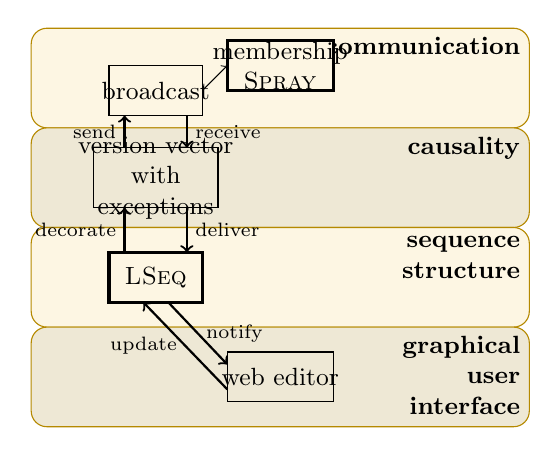
\begin{tikzpicture}[scale=0.9]

\newcommand\X{25pt}
\newcommand\Y{20pt}

\newcommand\LIGHTERGRAY{base3}
\newcommand\LIGHTGRAY{base2}
\newcommand\MEDIUMGRAY{yellow}

\small
%% communication
\draw[rounded corners=2mm, color=\MEDIUMGRAY, fill=\LIGHTERGRAY](0pt, 0pt)+(-4*\X,-\Y)rectangle+(4*\X,\Y);
\draw(4*\X, \Y)node[anchor=north east]{\textbf{communication}};

\draw[fill=\LIGHTERGRAY](-2*\X, -0.25*\Y)
node{broadcast}+(-0.75*\X,-0.5*\Y)rectangle+(0.75*\X,0.5*\Y);
\draw[fill=\LIGHTERGRAY, very thick]( 0*\X, 0.25*\Y)
node[align=center]{membership\\\SPRAY}+(-0.85*\X,-0.5*\Y)rectangle+(0.85*\X,0.5*\Y);
%%\draw[fill=white]( 2*\X, -0.25*\Y)
%% node{unicast}+(-0.75*\X,-0.5*\Y)rectangle+(0.75*\X,0.5*\Y);

\draw[<-](-0.85*\X, 0.25*\Y)--(-1.25*\X, -0.25*\Y);
%% \draw[<-](0.85*\X, 0.25*\Y)--(1.25*\X, -0.25*\Y);

%% causality
\draw[rounded corners=2mm, color=\MEDIUMGRAY, fill=\LIGHTGRAY](0pt, -2*\Y)+(-4*\X,-\Y)rectangle+(4*\X,\Y);
\draw(4*\X, -\Y)node[anchor=north east]{\textbf{causality}};

\draw[fill=\LIGHTGRAY](-2*\X, -2*\Y)
node[align=center]{version vector\\with\\exceptions}
+(-1.0*\X,-0.6*\Y)rectangle+(1.0*\X,0.6*\Y);
\scriptsize
\draw[->, thick](-1.5*\X, -0.75*\Y) -- node[anchor=west]{receive}
(-1.5*\X, -1.4*\Y);
\draw[<-, thick](-2.5*\X, -0.75*\Y) -- node[anchor=east]{send}
(-2.5*\X, -1.4*\Y);
\small
%% \draw[<->]( 2*\X, -0.75*\Y)--( 1*\X, -2.5*\Y);

%% sequence structure
\draw[rounded corners=2mm, color=\MEDIUMGRAY, fill=\LIGHTERGRAY](0pt, -4*\Y)+(-4*\X,-\Y)rectangle+(4*\X,\Y);
\draw(4*\X, -3*\Y)node[anchor=north east, align=right]
{\textbf{sequence}\\\textbf{structure}};

%% \draw[fill=white, shading=axis,top color=\LIGHTGRAY, bottom color=white, shading angle=0](1*\X, -3*\Y)
%% node{anti-entropy}+(-0.95*\X,-0.5*\Y) rectangle +(0.95 *\X, 0.5*\Y);
\draw[fill=\LIGHTERGRAY, very thick](-2*\X, -4*\Y)
node{\LSEQ}+(-0.75*\X,-0.5*\Y) rectangle +(0.75 *\X, 0.5*\Y);

%\draw[->] (0.05*\X, -2.75*\Y)--(-1*\X,-2*\Y);
%\draw[->] (0.05*\X, -3.25*\Y)--(-1.25*\X,-4*\Y);
\scriptsize
\draw[<-, thick] (-1.5*\X, -3.5*\Y)--node[anchor=west]{deliver}(-1.5*\X, -2.6*\Y);
\draw[->, thick] (-2.5*\X, -3.5*\Y)--node[anchor=east]{decorate}(-2.5*\X, -2.6*\Y);
\small
%% gui
\draw[rounded corners=2mm, color=\MEDIUMGRAY, fill=\LIGHTGRAY](0pt, -6*\Y)+(-4*\X,-\Y)rectangle+(4*\X,\Y);
\draw(4*\X, -5*\Y)node[anchor=north east, align=right]
{\textbf{graphical}\\\textbf{user}\\\textbf{interface}};
\draw[fill=\LIGHTGRAY](0pt,-6*\Y)
node{web editor}+(-0.85*\X,-0.5*\Y) rectangle +(0.85 *\X, 0.5*\Y);

%%\draw[<->] (-2*\X, -4.5*\Y) -- (0*\X, -5.5*\Y);
\scriptsize
\draw[->, thick] (-1.80*\X, -4.5*\Y)--node[anchor=west]{notify}(-0.85*\X, -5.75*\Y);
\draw[<-, thick] (-2.20*\X, -4.5*\Y)--node[anchor=east]{update}(-0.85*\X, -6.25*\Y);
\small
\end{tikzpicture}
  }
  
  \headerbox{\textsc{Network of Browsers}}
  {name=network, column=1, span=1, below=objective}{
    
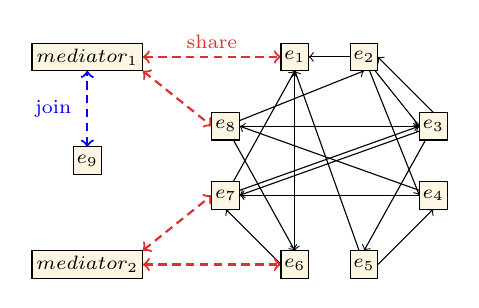
\begin{tikzpicture}[scale=1]

  \newcommand\X{25pt}
  \newcommand\Y{-25pt}

  \draw[->] (\X, 0)--(\X, 5+3*\Y); %% p1 p6
  \draw[->] (-5+2*\X, 0)--(5+\X, 0); %% p2 p1
  \draw[->] (2*\X, 0) -- (-5+3*\X, \Y); %% p2 p3
  \draw[->] (2*\X, 0) -- (-5+3*\X, 2*\Y); %% p2 p4
  \draw[->] (3*\X, 5+\Y) -- ( 5+2*\X, 0); %% p3 p2
  \draw[->] (3*\X, \Y) -- (5pt, 2*\Y); %% p3 p7
  \draw[->] (3*\X, \Y) -- (2*\X, 5+3*\Y); %% p3 p5
  \draw[->] (3*\X, 2*\Y) -- (5pt, 2*\Y); %% p4 p7
  \draw[->] (3*\X, 2*\Y) -- (5pt, \Y); %% p4 p8
  \draw[->] (2*\X, 3*\Y) -- (\X, -5pt); %% p5 p1
  \draw[->] (5+2*\X, 3*\Y) -- (3*\X, -5+ 2*\Y); %% p5 p4
  \draw[->] (-5+\X, 3*\Y) -- (0pt, -5+2*\Y); %% p6 p7
  \draw[->] (0pt, 2*\Y) -- (-5+3*\X, \Y); %% p7 p3
  \draw[->] (0pt, 2*\Y) -- (\X, -5pt); %% p7 p1
  \draw[->] (0pt, \Y) -- (2*\X, -5pt); %% p8 p2
  \draw[->] (0pt, \Y) -- (\X, 5+3*\Y); %% p8 p6
  \draw[->] (0pt, \Y) -- (-5+3*\X, \Y); %% p8 p3
  
  \scriptsize
  \draw[fill=base3] (-2*\X, 1.5*\Y) node{$e_9$} +(-5pt,-5pt) rectangle +(5pt,5pt);
  \draw[<->, densely dashed, color=blue, thick] (-2*\X, 5+1.5*\Y) -- node[anchor=east]{join \ } (-2*\X, -5pt);

  \draw[fill=base3] (-2*\X, 0) node{$mediator_1$} +(-20pt, -5pt)rectangle+(20pt, 5pt);
  \draw[<->, densely dashed, color=red, thick] (20-2*\X, 0) -- node[anchor=south]{share} (-5+\X, 0);
  \draw[<->, densely dashed, color=red, thick] (20-2*\X, -5pt) -- (-5pt, \Y);
  
  \draw[fill=base3] (-2*\X, 3*\Y) node{$mediator_2$} +(-20pt, -5pt)rectangle+(20pt, 5pt);
  \draw[<->, densely dashed, color=red, thick] (20-2*\X, 3*\Y) -- (-5+\X, 3*\Y);
  \draw[<->, densely dashed, color=red, thick] (20-2*\X, 5+3*\Y) -- (-5pt, 2*\Y);

  \draw[fill=base3] (\X, 0)node{$e_1$}+(-5pt, -5pt)rectangle+(5pt, 5pt);
  \draw[fill=base3] (2*\X, 0)node{$e_2$}+(-5pt, -5pt)rectangle+(5pt, 5pt);
  \draw[fill=base3] (3*\X, \Y)node{$e_3$}+(-5pt, -5pt)rectangle+(5pt, 5pt);
  \draw[fill=base3] (3*\X, 2*\Y)node{$e_4$}+(-5pt, -5pt)rectangle+(5pt, 5pt);
  \draw[fill=base3] (2*\X, 3*\Y)node{$e_5$}+(-5pt, -5pt)rectangle+(5pt, 5pt);
  \draw[fill=base3] (1*\X, 3*\Y)node{$e_6$}+(-5pt, -5pt)rectangle+(5pt, 5pt);
  \draw[fill=base3] (0 , 2*\Y)node{$e_7$}+(-5pt, -5pt)rectangle+(5pt, 5pt);
%  \draw[fill=base3] (0 , \Y)+(-55pt, -10pt)rectangle+(5pt, 10pt);
  \draw[fill=base3](0,\Y) node{$e_8$}+(-5pt, -5pt)rectangle+(5pt, 5pt);

\end{tikzpicture}
  }

  \headerbox{\textsc{Distributed Structure}}
  {name=structure, column=2, span=1, below=objective}{
    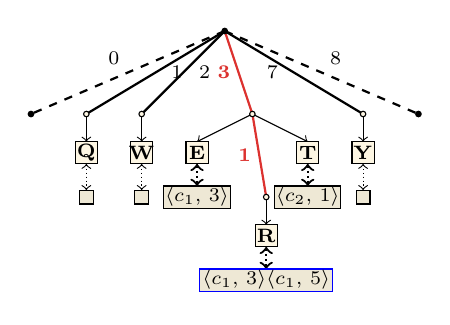
\begin{tikzpicture}[scale=1]

\newcommand\Y{-30};
\newcommand\ADDY{-10};

  %% node to node
  \scriptsize
  \draw[dashed,thick] (0pt,0pt) -- node[anchor=south east]{0} (-70pt,\Y pt);
  \draw[thick] (0pt,0pt) -- node[anchor=west]{\ 1} (-50pt, \Y pt); %% Q
  \draw[thick] (0pt,0pt) -- node[anchor=west]{\ 2} (-30pt, \Y pt); %% W
  \draw[thick,color=red] (0pt,0pt) -- node[anchor=east]{\textbf{3}}
  (  10pt, \Y pt); %% E R
  \draw[thick,color=red] (10pt,\Y pt) -- node[anchor=east]{\textbf{1}}
  ( 15pt, 2*\Y pt); %% T
  \draw[thick] (0pt,0pt) -- node[anchor=east]{7 \ } ( 50pt, \Y pt); %% Y
  \draw[dashed,thick] (0pt,0pt) -- node[anchor=south west]{8} ( 70pt, \Y pt);

  %% node to element
  \draw[->] (-50pt,\Y pt) -- (-50pt, \ADDY +\Y pt);
  \draw[->] (-30pt,\Y pt) -- (-30pt, \ADDY +\Y pt);
  \draw[->] (  10pt,\Y pt) -- (-10pt, \ADDY +\Y pt);
  \draw[->] (  10pt,\Y pt) -- ( 30pt, \ADDY +\Y pt);
  \draw[->] (  15pt,2*\Y pt) -- ( 15pt, \ADDY + 2*\Y pt);
  \draw[->] ( 50pt,\Y pt) -- ( 50pt, \ADDY +\Y pt);

  %% element to desambiguator
  \draw[<->,densely dotted](-50pt,-8+\ADDY + \Y pt)--(-50pt,2.75*\ADDY+\Y pt);
  \draw[<->,densely dotted](-30pt,-8+\ADDY + \Y pt)--(-30pt,2.75*\ADDY+\Y pt);
  \draw[<->,densely dotted, thick](-10pt,-8+\ADDY + \Y pt)--(-10pt,2.6*\ADDY+\Y pt);
  \draw[<->,densely dotted, thick](15pt,-8+\ADDY + 2*\Y pt)--(15pt,2.6*\ADDY+2*\Y pt);
  \draw[<->,densely dotted, thick]( 30pt,-8+\ADDY + \Y pt)--( 30pt,2.6*\ADDY+\Y pt);
  \draw[<->,densely dotted]( 50pt,-8+\ADDY + \Y pt)--( 50pt,2.75*\ADDY+\Y pt);

  %% nodes
  \draw[fill=black] ( 0pt, 0 pt) circle (1pt); 
  \draw[fill=black] (-70pt, \Y pt) circle (1pt); 
  \draw[fill=base3] (-50pt, \Y pt) circle (1pt); %% Q
  \draw[fill=base3] (-30pt, \Y pt) circle (1pt); %% W
  \draw[fill=base3] ( 10pt, \Y pt) circle (1pt); %% E
  \draw[fill=base3] ( 15pt, 2*\Y pt) circle (1pt); %% T
  \draw[fill=base3] ( 50pt, \Y pt) circle (1pt); %% Y
  \draw[fill=black] ( 70pt, \Y pt) circle (1pt);

  %% desambiguator
  \draw[fill=base2] (-50pt,-2.5+2.75*\ADDY+\Y pt)
  +(-2.5pt,-2.5pt) rectangle +(2.5pt,2.5pt);
  \draw[fill=base2] (-30pt,-2.5+2.75*\ADDY+\Y pt)
  +(-2.5pt,-2.5pt) rectangle +(2.5pt,2.5pt);
  \draw[fill=base2] (-10pt,-2.5+2.75*\ADDY+\Y pt)
  node{$\langle c_1,\, 3\rangle$}
  +(-12pt,-4pt) rectangle +(12pt,4pt);
  \draw[fill=base2, draw=blue] ( 15pt,-2.5+2.75*\ADDY+2*\Y pt)
  node{\BLUE{$\langle c_1,\, 3\rangle\langle c_1,\,5\rangle$}}
  +(-24pt,-4pt) rectangle +(24pt,4pt);
  \draw[fill=base2] ( 30pt,-2.5+2.75*\ADDY+\Y pt)
  node{$\langle c_2,\, 1\rangle$}
  +(-12pt,-4pt) rectangle +(12pt,4pt);
  \draw[fill=base2] ( 50pt,-2.5+2.75*\ADDY+\Y pt)
  +(-2.5pt,-2.5pt) rectangle +(2.5pt,2.5pt);

  %% elements
  \draw[fill=base3](-50pt,-4 + \ADDY + \Y pt)
  node{\textbf{Q}} +(-4pt,-4pt) rectangle +(4pt,4pt) ; %% Q
  \draw[fill=base3](-30pt,-4 + \ADDY + \Y pt)
  node{\textbf{W}} +(-4pt,-4pt) rectangle +(4pt,4pt) ; %% W
  \draw[fill=base3](- 10pt,-4 + \ADDY + \Y pt)
  node{\textbf{E}} +(-4pt,-4pt) rectangle +(4pt,4pt) ; %% E
  \draw[fill=base3]( 15pt,-4 + \ADDY + 2*\Y pt)
  node{\textbf{R}} +(-4pt,-4pt) rectangle +(4pt,4pt) ; %% R
  \draw[fill=base3]( 30pt,-4 + \ADDY + \Y pt)
  node{\textbf{T}} +(-4pt,-4pt) rectangle +(4pt,4pt) ; %% T
  \draw[fill=base3]( 50pt,-4 + \ADDY + \Y pt)
  node{\textbf{Y}} +(-4pt,-4pt) rectangle +(4pt,4pt) ; %% Y

  
  % \begin{scope}[shift={(20pt, 2.5*\Y pt)}]    
  %   \draw[fill=base3](0,0)node{\textbf{E}} +(-4pt, -4pt) rectangle +(4pt, 4pt);
  %   \scriptsize
  %   \draw (4pt, 0)node[anchor=west]{element};
  %   \draw[fill=base2] (0,\ADDY pt) +(-2.5pt, -2.5pt)rectangle+(2.5pt, 2.5pt);
  %   \draw (3pt, \ADDY pt) node[anchor=west]{disambiguator};
  % \end{scope}
  %% spacing
  \draw(0, -8+\ADDY+ 2.6*\Y pt);

\end{tikzpicture}

  }

  \headerbox{\textsc{Result}}
  {name=result, column=0, span=1, below=architecture}{
    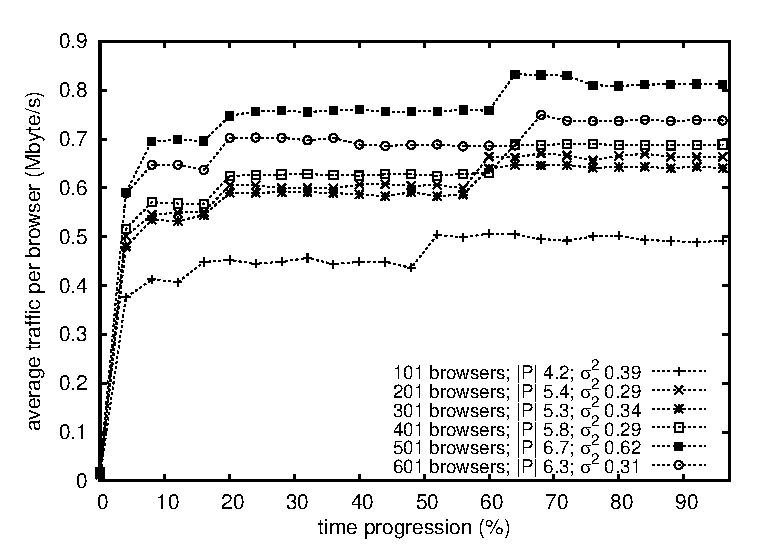
\includegraphics[scale=0.4]{img/traffic.eps}
  }

  \headerbox{\textsc{Conclusion}}
  {name=conclusion, column=1, span=1, below=architecture}{
  }

  \headerbox{\textsc{Session WWW}}
  {name=session, column=2, below=architecture} {
    \centering
    
\includegraphics[scale=0.25]{img/qrcode.png}
    or\\
    \url{chat-wane.github.io/CRATE/?www}
  }

\end{poster}


\end{document}

